% Drawing 74/04-13 -- folder 74, batch 04, archive page 77 (PDF page 78).
% Transcription: en haut à gauche, au crayon, un hexagone dont trois côtés alternés sont repassés en gras, avec ses diagonales tracées légèrement ; deux sommets opposés sont marqués d'un gros point.
% Kind: hexagon with its diagonals, alternate sides heavy. Method 2 (schematic redraw from the facsimile). Status: partial.
% Notes: Top left of the sheet, pencil; the left third of the crop. A hexagon on six vertices placed once; three alternate sides gone over heavily, the other three light; the nine diagonals (the three long ones and the two inscribed triangles) in light pencil between the same vertices; two opposite vertices carry a heavy point. Below the hexagon a point, a small cross and a dot are left out. Still differs: the pencil diagonals overlap and cannot all be told apart at this resolution, all nine are drawn (he lists the diagonals and the inscribed triangles of the hexagon on this page); small crosses that may mark the other four vertices are left out. Id 04-13: existing ids are not renumbered. Redrawn 2026-11-12 (issue 128): to check again.
% Coordinates: 1 unit = 1 mm = 1/100 of the crop width (bbox in page fractions: [0.15, 0.085, 0.36, 0.16]).
% Redrawn by Claude (claude-fable-5-2), issue #128, 2026-11-12; not checked by a human; not compiled (no TeX in the session).
% Rights: reproduces part of the work -- behind RENDER_TRANSCRIPTS, never published by itself.
\documentclass[tikz,border=3pt]{standalone}
\usepackage{amsmath,amssymb}
\usetikzlibrary{patterns,arrows.meta}
\tikzset{pencil/.style={black!45}, struck/.style={black!35}, mpt/.style={circle,draw,inner sep=1.3pt}, pt/.style={circle,fill,inner sep=0.9pt}, opt/.style={circle,draw,fill=white,inner sep=1.1pt}}
\begin{document}
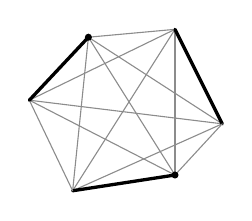
\begin{tikzpicture}[x=1mm,y=1mm,line cap=round,line join=round,font=\small]
\coordinate (V1) at (18,-10.5);
\coordinate (V2) at (29,-9.5);
\coordinate (V3) at (35,-21.5);
\coordinate (V4) at (29,-28);
\coordinate (V5) at (16,-30);
\coordinate (V6) at (10.5,-18.5);
\draw[pencil,thin] (V1) -- (V3);
\draw[pencil,thin] (V1) -- (V4);
\draw[pencil,thin] (V1) -- (V5);
\draw[pencil,thin] (V2) -- (V4);
\draw[pencil,thin] (V2) -- (V5);
\draw[pencil,thin] (V2) -- (V6);
\draw[pencil,thin] (V3) -- (V5);
\draw[pencil,thin] (V3) -- (V6);
\draw[pencil,thin] (V4) -- (V6);
\draw[pencil] (V1) -- (V2);
\draw[very thick] (V2) -- (V3);
\draw[pencil] (V3) -- (V4);
\draw[very thick] (V4) -- (V5);
\draw[pencil] (V5) -- (V6);
\draw[very thick] (V6) -- (V1);
\node[pt] at (V1) {};
\node[pt] at (V4) {};
\end{tikzpicture}
\end{document}
